\documentclass{standalone}
\usepackage{tikzducks}

\begin{document}
	
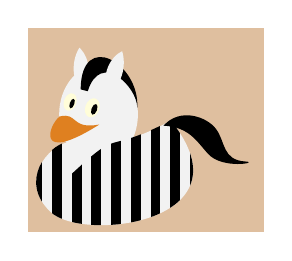
\begin{tikzpicture}
	\fill[brown!50!white] (0,0) rectangle (3,2.6);
	\begin{scope}[yshift=-6]
		\clip[rotate=-5] (0.68,2.38) ellipse (0.3 and 0.4);
		\fill[gray!10!white,rotate=-5] (0.28,2.26) ellipse (0.3 and 0.4);
	\end{scope}
	\duck[
		body=gray!10!white,
		stripes={\stripes[distance=0.25,width=0.125,rotate=0,initialx=0.06]},
		horsetail,
		mohican=black
	]
	\begin{scope}[yshift=-5,xshift=1]
		\clip[rotate=-5] (0.68,2.38) ellipse (0.3 and 0.4);
		\fill[gray!10!white,rotate=-5] (1.06,2.2) ellipse (0.3 and 0.4);
	\end{scope}
\end{tikzpicture}
	
\end{document}